 

\documentclass[12pt]{article}
%%%%%%%%%%%%%%%%%%%%%%%%%%%%%%%%%%%%%%%%%%%%%%%%%%%%%%%%%%%%%%%%%%%%%%%%%%%%%%%%%%%%%%%%%%%%%%%%%%%%%%%%%%%%%%%%%%%%%%%%%%%%%%%%%%%%%%%%%%%%%%%%%%%%%%%%%%%%%%%%%%%%%%%%%%%%%%%%%%%%%%%%%%%%%%%%%%%%%%%%%%%%%%%%%%%%%%%%%%%%%%%%%%%%%%%%%%%%%%%%%%%%%%%%%%%%
\usepackage{amsfonts}
\usepackage{eurosym}
\usepackage{geometry}
\usepackage{amsmath,amsthm,amssymb}
\usepackage{graphicx}
\usepackage{comment}
\usepackage{adjustbox}
\usepackage{array}
\usepackage{multirow}
\usepackage{subcaption}
\usepackage{pifont}
\usepackage{amssymb}
\usepackage{comment}
\usepackage[utf8]{inputenc}
\usepackage{setspace}
\usepackage[hang, flushmargin, bottom]{footmisc}
%\usepackage[backend=biber,style=apa,url=false,isbn=false, extra = false]{biblatex}

%\addbibresource{references.bib}
\usepackage{footnotebackref}
\usepackage{xcolor}
\usepackage{hyperref}
\usepackage{booktabs}
\usepackage{pifont}
\usepackage{caption}
\usepackage{float}


\setlength{\textfloatsep}{5pt}
\captionsetup{font=normalsize}
\newcommand{\cmark}{\ding{51}}
\def\sym#1{\ifmmode^{#1}\else\(^{#1}\)\fi}
\renewcommand{\thetable}{\Roman{table}}
\geometry{verbose,tmargin=.5in,bmargin=.7in,lmargin=.7in,rmargin=.7in,nomarginpar}
\makeatletter

\begin{document}

\title{Initial empirical results from SCOMP data}

\maketitle

In this document I will present what we are learnign from out empirical work. This is the continuation of the file which presents the initial datawork. 

\section{IE 4}

\subsection{Elasticity of shoppers vs non-shoppers}

The following table shows the coefficients of a conditional logit to test whether customers that ask for an external offer are more price elastic. Odd (even) columns run the specification on the sample with(without) external offers, which we think of as shoppers (non-shoppers). Once we control by the company fixed effects the shopers are more elastic. 

\begin{table}[htbp]\centering
\def\sym#1{\ifmmode^{#1}\else\(^{#1}\)\fi}
\caption{ratio on controls by rank\_sales}
\begin{tabular}{l*{8}{c}}
\hline\hline
                    &\multicolumn{1}{c}{(1)}&\multicolumn{1}{c}{(2)}&\multicolumn{1}{c}{(3)}&\multicolumn{1}{c}{(4)}&\multicolumn{1}{c}{(5)}&\multicolumn{1}{c}{(6)}&\multicolumn{1}{c}{(7)}&\multicolumn{1}{c}{(8)}\\
                    &\multicolumn{1}{c}{ratio}&\multicolumn{1}{c}{ratio}&\multicolumn{1}{c}{ratio}&\multicolumn{1}{c}{ratio}&\multicolumn{1}{c}{ratio}&\multicolumn{1}{c}{ratio}&\multicolumn{1}{c}{ratio}&\multicolumn{1}{c}{ratio}\\
\hline
val\_uf\_prima2       &         0.2\sym{***}&         1.4\sym{***}&         0.4\sym{***}&         0.3\sym{***}&         0.3\sym{***}&         1.0\sym{***}&         0.1\sym{*}  &         0.1         \\
                    &       (0.1)         &       (0.1)         &       (0.1)         &       (0.1)         &       (0.1)         &       (0.1)         &       (0.1)         &       (0.1)         \\
[1em]
male                &        -8.8\sym{***}&       -10.7\sym{***}&        -9.9\sym{***}&        -7.5\sym{***}&        -8.2\sym{***}&       -10.7\sym{***}&        -7.7\sym{***}&        -6.6\sym{***}\\
                    &       (0.3)         &       (0.3)         &       (0.3)         &       (0.3)         &       (0.3)         &       (0.4)         &       (0.4)         &       (0.4)         \\
[1em]
age\_years           &        -5.7\sym{***}&        -5.5\sym{***}&        -5.8\sym{***}&        -6.1\sym{***}&        -5.9\sym{***}&        -5.5\sym{***}&        -5.6\sym{***}&        -5.7\sym{***}\\
                    &       (0.0)         &       (0.0)         &       (0.0)         &       (0.0)         &       (0.0)         &       (0.1)         &       (0.1)         &       (0.1)         \\
[1em]
A                   &         0.0         &         0.0         &         0.0         &         0.0         &         0.0         &         0.0         &         0.0         &         0.0         \\
                    &         (.)         &         (.)         &         (.)         &         (.)         &         (.)         &         (.)         &         (.)         &         (.)         \\
[1em]
D                   &        -1.0\sym{***}&        -1.3\sym{***}&        -1.5\sym{***}&        -0.7\sym{**} &        -0.7\sym{**} &        -0.4         &        -0.2         &         0.2         \\
                    &       (0.3)         &       (0.3)         &       (0.3)         &       (0.3)         &       (0.3)         &       (0.4)         &       (0.3)         &       (0.4)         \\
[1em]
P                   &        -0.1         &        -0.3         &        -0.2         &        -1.0\sym{**} &         0.1         &        -0.2         &         0.1         &         0.0         \\
                    &       (0.4)         &       (0.3)         &       (0.4)         &       (0.4)         &       (0.4)         &       (0.5)         &       (0.4)         &       (0.5)         \\
[1em]
Constant            &       577.1\sym{***}&       563.8\sym{***}&       587.4\sym{***}&       601.6\sym{***}&       587.7\sym{***}&       559.2\sym{***}&       564.0\sym{***}&       573.0\sym{***}\\
                    &       (3.0)         &       (2.9)         &       (2.8)         &       (3.0)         &       (2.8)         &       (3.6)         &       (4.6)         &       (3.2)         \\
\hline
N                   &     18266.0         &     20151.0         &     21324.0         &     13485.0         &     19945.0         &     11870.0         &     10148.0         &      9475.0         \\
R-sq                &         0.7         &         0.7         &         0.6         &         0.7         &         0.7         &         0.6         &         0.7         &         0.7         \\
\hline\hline
\multicolumn{9}{l}{\footnotesize Standard errors in parentheses}\\
\multicolumn{9}{l}{\footnotesize \sym{*} \(p<0.10\), \sym{**} \(p<0.05\), \sym{***} \(p<0.01\)}\\
\end{tabular}
\end{table}

 \newpage 
 
 \begin{table}[htbp]\centering
\def\sym#1{\ifmmode^{#1}\else\(^{#1}\)\fi}
\caption{ratio on controls by rank\_sales}
\begin{tabular}{l*{8}{c}}
\hline\hline
                    &\multicolumn{1}{c}{(1)}&\multicolumn{1}{c}{(2)}&\multicolumn{1}{c}{(3)}&\multicolumn{1}{c}{(4)}&\multicolumn{1}{c}{(5)}&\multicolumn{1}{c}{(6)}&\multicolumn{1}{c}{(7)}&\multicolumn{1}{c}{(8)}\\
                    &\multicolumn{1}{c}{ratio}&\multicolumn{1}{c}{ratio}&\multicolumn{1}{c}{ratio}&\multicolumn{1}{c}{ratio}&\multicolumn{1}{c}{ratio}&\multicolumn{1}{c}{ratio}&\multicolumn{1}{c}{ratio}&\multicolumn{1}{c}{ratio}\\
\hline
male                &      -8.882\sym{***}&     -11.263\sym{***}&     -10.035\sym{***}&      -7.570\sym{***}&      -8.290\sym{***}&      -9.611\sym{***}&      -7.764\sym{***}&      -6.569\sym{***}\\
                    &     (0.299)         &     (0.290)         &     (0.291)         &     (0.323)         &     (0.302)         &     (0.402)         &     (0.387)         &     (0.356)         \\
[1em]
age\_years           &      -5.684\sym{***}&      -5.271\sym{***}&      -5.722\sym{***}&      -6.027\sym{***}&      -5.879\sym{***}&      -5.338\sym{***}&      -5.532\sym{***}&      -5.664\sym{***}\\
                    &     (0.044)         &     (0.045)         &     (0.043)         &     (0.046)         &     (0.044)         &     (0.057)         &     (0.072)         &     (0.050)         \\
[1em]
A                   &       0.000         &       0.000         &       0.000         &       0.000         &       0.000         &       0.000         &       0.000         &       0.000         \\
                    &         (.)         &         (.)         &         (.)         &         (.)         &         (.)         &         (.)         &         (.)         &         (.)         \\
[1em]
D                   &      -0.970\sym{***}&      -0.944\sym{***}&      -1.382\sym{***}&      -0.611\sym{**} &      -0.614\sym{**} &      -0.248         &      -0.164         &       0.206         \\
                    &     (0.282)         &     (0.267)         &     (0.271)         &     (0.303)         &     (0.285)         &     (0.360)         &     (0.313)         &     (0.357)         \\
[1em]
P                   &       0.014         &       0.132         &      -0.080         &      -0.873\sym{**} &       0.186         &      -0.005         &       0.138         &       0.019         \\
                    &     (0.375)         &     (0.353)         &     (0.358)         &     (0.414)         &     (0.377)         &     (0.473)         &     (0.410)         &     (0.456)         \\
[1em]
Constant            &     575.315\sym{***}&     552.213\sym{***}&     583.787\sym{***}&     599.686\sym{***}&     585.535\sym{***}&     552.407\sym{***}&     563.024\sym{***}&     572.529\sym{***}\\
                    &     (2.937)         &     (2.879)         &     (2.734)         &     (2.943)         &     (2.781)         &     (3.625)         &     (4.546)         &     (3.205)         \\
\hline
N                   &   18266.000         &   20151.000         &   21324.000         &   13485.000         &   19945.000         &   11870.000         &   10148.000         &    9475.000         \\
R-sq                &       0.657         &       0.645         &       0.645         &       0.708         &       0.655         &       0.643         &       0.662         &       0.717         \\
\hline\hline
\multicolumn{9}{l}{\footnotesize Standard errors in parentheses}\\
\multicolumn{9}{l}{\footnotesize \sym{*} \(p<0.10\), \sym{**} \(p<0.05\), \sym{***} \(p<0.01\)}\\
\end{tabular}
\end{table}

 

 
\subsection{Firms using more-less external offers}

\begin{figure}[H]
\caption{}
 \label{fig:ie4_1}
\centering{}%
\begin{tabular}{cc}
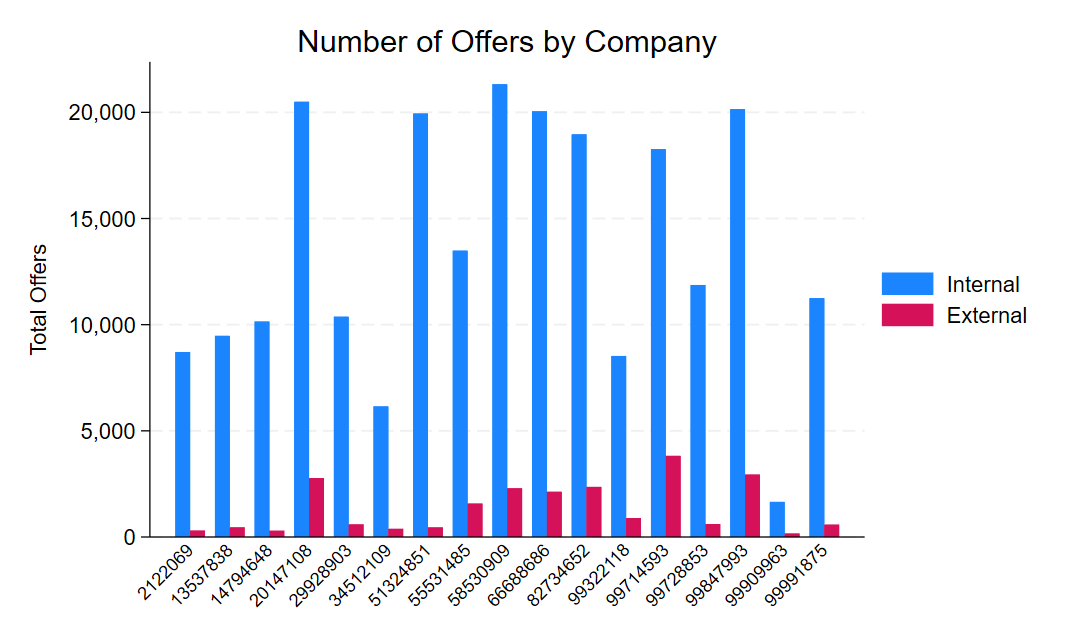
\includegraphics[scale=0.17]{figures/IE4/IE4_int_ext_offers_by_cia.png} 
\end{tabular}
\end{figure}

   

\end{document}